% generated by gen_amo_fig.py -- do not edit by hand
\documentclass[10pt]{standalone}
\usepackage{helvet}
\renewcommand{\familydefault}{\sfdefault}
\usepackage{amsmath,amssymb}
\usepackage{tikz}
\usetikzlibrary{arrows.meta}
\definecolor{cctrl}{HTML}{D6E0EC}
\definecolor{cctrlb}{HTML}{3B5675}
\definecolor{cexe}{HTML}{FFE699}
\definecolor{cexeb}{HTML}{7F6000}
\definecolor{cmem}{HTML}{FBE5D6}
\definecolor{cmemb}{HTML}{C55A11}
\definecolor{csto}{HTML}{E2EFDA}
\newcommand{\fs}{\fontsize{6.4}{7.4}\selectfont}
\newcommand{\fss}{\fontsize{5.8}{6.6}\selectfont}
\begin{document}
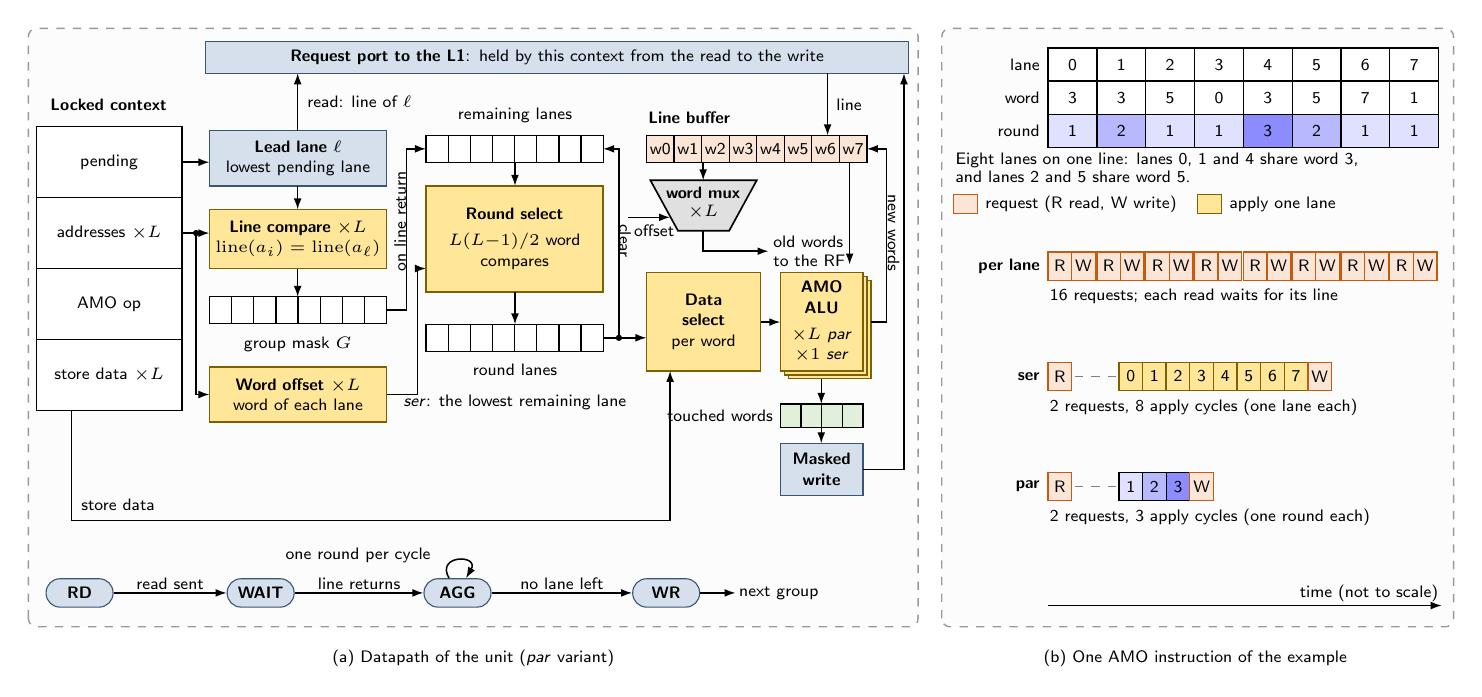
\begin{tikzpicture}[x=1cm, y=1cm,
  base/.style={align=center, font=\fs, inner sep=1pt, line width=0.5pt},
  ctrl/.style={base, draw=cctrlb, fill=cctrl},
  exe/.style={base, draw=cexeb, fill=cexe},  exebox/.style={draw=cexeb, fill=cexe, line width=0.5pt},
  membox/.style={draw=cmemb, fill=cmem, line width=0.5pt},
  mux/.style={draw=black, fill=black!12, line width=0.6pt},
  tbl/.style={draw=black, line width=0.45pt},
  cell/.style={font=\fss, inner sep=0.5pt}, cellh/.style={font=\fss\bfseries, inner sep=0.5pt},
  tbltitle/.style={font=\fs, inner sep=0.5pt},
  panel/.style={draw=black!40, dashed, rounded corners=3pt, fill=black!1, line width=0.5pt},
  fsm/.style={draw=cctrlb, fill=cctrl, rounded corners=5pt, font=\fss\bfseries,
              minimum width=0.85cm, minimum height=0.36cm, inner sep=1pt},
  lbl/.style={font=\fs, inner sep=0.5pt},
  wlabel/.style={font=\fss, inner sep=1pt},
  keytext/.style={font=\fss, inner sep=0.5pt},
  subcap/.style={font=\fs, inner sep=1pt},
  vlabel/.style={font=\fss, rotate=90, inner sep=0.5pt},
  vlabelr/.style={font=\fss, rotate=-90, inner sep=0.5pt},
  arr/.style={-{Latex[length=1.4mm, width=1.0mm]}, line width=0.55pt}]
\draw[panel] (-0.100,-0.050) rectangle (11.200,7.550);
\node[ctrl, minimum width=8.930cm, minimum height=0.400cm, text width=8.830cm] at (6.615,7.180) {\textbf{Request port to the L1}: held by this context from the read to the write};
\node[tbltitle, anchor=center] at (0.920,6.580) {\textbf{Locked context}};
\draw[tbl, fill=white] (0.000,5.400) rectangle (1.850,6.300);
\node[cell, anchor=center] at (0.925,5.850) {pending};
\draw[tbl, fill=white] (0.000,4.500) rectangle (1.850,5.400);
\node[cell, anchor=center] at (0.925,4.950) {addresses $\times L$};
\draw[tbl, fill=white] (0.000,3.600) rectangle (1.850,4.500);
\node[cell, anchor=center] at (0.925,4.050) {AMO op};
\draw[tbl, fill=white] (0.000,2.700) rectangle (1.850,3.600);
\node[cell, anchor=center] at (0.925,3.150) {store data $\times L$};
\node[ctrl, minimum width=2.250cm, minimum height=0.700cm, text width=2.150cm] at (3.325,5.900) {\textbf{Lead lane} $\ell$\\lowest pending lane};
\node[exe, minimum width=2.250cm, minimum height=0.750cm, text width=2.150cm] at (3.325,4.875) {\textbf{Line compare} $\times L$\\$\mathrm{line}(a_i)=\mathrm{line}(a_\ell)$};
\draw[tbl, fill=white] (2.200,3.800) rectangle (2.481,4.140);
\draw[tbl, fill=white] (2.481,3.800) rectangle (2.763,4.140);
\draw[tbl, fill=white] (2.763,3.800) rectangle (3.044,4.140);
\draw[tbl, fill=white] (3.044,3.800) rectangle (3.325,4.140);
\draw[tbl, fill=white] (3.325,3.800) rectangle (3.606,4.140);
\draw[tbl, fill=white] (3.606,3.800) rectangle (3.888,4.140);
\draw[tbl, fill=white] (3.888,3.800) rectangle (4.169,4.140);
\draw[tbl, fill=white] (4.169,3.800) rectangle (4.450,4.140);
\node[cell, anchor=north] at (3.320,3.660) {group mask $G$};
\node[exe, minimum width=2.250cm, minimum height=0.700cm, text width=2.150cm] at (3.325,2.900) {\textbf{Word offset} $\times L$\\word of each lane};
\draw[arr] (1.850,5.850) -- (2.200,5.850);
\draw[arr] (1.850,4.950) -- (2.200,4.950);
\fill (2.030,4.950) circle (0.04);
\draw[arr] (2.030,4.950) -- (2.030,2.900) -- (2.200,2.900);
\draw[arr] (3.320,5.550) -- (3.320,5.250);
\draw[arr] (3.320,4.500) -- (3.320,4.140);
\draw[arr] (3.320,6.250) -- (3.320,6.980);
\node[wlabel, anchor=west] at (3.400,6.620) {read: line of $\ell$};
\draw[tbl, fill=white] (4.950,5.850) rectangle (5.231,6.190);
\draw[tbl, fill=white] (5.231,5.850) rectangle (5.513,6.190);
\draw[tbl, fill=white] (5.513,5.850) rectangle (5.794,6.190);
\draw[tbl, fill=white] (5.794,5.850) rectangle (6.075,6.190);
\draw[tbl, fill=white] (6.075,5.850) rectangle (6.356,6.190);
\draw[tbl, fill=white] (6.356,5.850) rectangle (6.638,6.190);
\draw[tbl, fill=white] (6.638,5.850) rectangle (6.919,6.190);
\draw[tbl, fill=white] (6.919,5.850) rectangle (7.200,6.190);
\node[cell, anchor=south] at (6.080,6.330) {remaining lanes};
\node[exe, minimum width=2.250cm, minimum height=1.350cm, text width=2.150cm] at (6.075,4.875) {\textbf{Round select}\\[2pt]$L(L{-}1)/2$ word\\compares};
\draw[tbl, fill=white] (4.950,3.450) rectangle (5.231,3.790);
\draw[tbl, fill=white] (5.231,3.450) rectangle (5.513,3.790);
\draw[tbl, fill=white] (5.513,3.450) rectangle (5.794,3.790);
\draw[tbl, fill=white] (5.794,3.450) rectangle (6.075,3.790);
\draw[tbl, fill=white] (6.075,3.450) rectangle (6.356,3.790);
\draw[tbl, fill=white] (6.356,3.450) rectangle (6.638,3.790);
\draw[tbl, fill=white] (6.638,3.450) rectangle (6.919,3.790);
\draw[tbl, fill=white] (6.919,3.450) rectangle (7.200,3.790);
\node[cell, anchor=north] at (6.080,3.310) {round lanes};
\node[cell, anchor=north] at (6.080,2.920) {\emph{ser}: the lowest remaining lane};
\draw[arr] (4.450,3.970) -- (4.700,3.970) -- (4.700,6.020) -- (4.950,6.020);
\node[vlabel, anchor=center] at (4.620,5.100) {on line return};
\draw[arr] (6.080,5.850) -- (6.080,5.550);
\draw[arr] (4.450,2.900) -- (4.840,2.900) -- (4.840,4.500) -- (4.950,4.500);
\draw[arr] (6.080,4.200) -- (6.080,3.790);
\fill (7.400,3.620) circle (0.04);
\draw[arr] (7.200,3.620) -- (7.400,3.620) -- (7.400,6.020) -- (7.200,6.020);
\node[vlabelr, anchor=center] at (7.480,4.850) {clear};
\node[tbltitle, anchor=west] at (7.750,6.420) {\textbf{Line buffer}};
\draw[tbl, fill=cmem] (7.750,5.850) rectangle (8.100,6.190);
\node[cell, anchor=center] at (7.925,6.020) {w0};
\draw[tbl, fill=cmem] (8.100,5.850) rectangle (8.450,6.190);
\node[cell, anchor=center] at (8.275,6.020) {w1};
\draw[tbl, fill=cmem] (8.450,5.850) rectangle (8.800,6.190);
\node[cell, anchor=center] at (8.625,6.020) {w2};
\draw[tbl, fill=cmem] (8.800,5.850) rectangle (9.150,6.190);
\node[cell, anchor=center] at (8.975,6.020) {w3};
\draw[tbl, fill=cmem] (9.150,5.850) rectangle (9.500,6.190);
\node[cell, anchor=center] at (9.325,6.020) {w4};
\draw[tbl, fill=cmem] (9.500,5.850) rectangle (9.850,6.190);
\node[cell, anchor=center] at (9.675,6.020) {w5};
\draw[tbl, fill=cmem] (9.850,5.850) rectangle (10.200,6.190);
\node[cell, anchor=center] at (10.025,6.020) {w6};
\draw[tbl, fill=cmem] (10.200,5.850) rectangle (10.550,6.190);
\node[cell, anchor=center] at (10.375,6.020) {w7};
\draw[arr] (10.050,6.980) -- (10.050,6.190);
\node[wlabel, anchor=west] at (10.120,6.580) {line};
\draw[mux] (7.80,5.62) -- (9.15,5.62) -- (8.80,4.98) -- (8.15,4.98) -- cycle;
\node[cell, align=center] at (8.47,5.33) {\textbf{word mux}\\$\times L$};
\draw[arr] (8.470,5.850) -- (8.470,5.620);
\draw[arr] (7.520,5.150) -- (8.050,5.150);
\node[wlabel, anchor=north west] at (7.550,5.100) {offset};
\draw[arr] (8.470,4.980) -- (8.470,4.720) -- (9.300,4.720);
\node[wlabel, anchor=west, align=left] at (9.32,4.72) {old words\\to the RF};
\node[exe, minimum width=1.450cm, minimum height=1.250cm, text width=1.350cm] at (8.475,3.825) {\textbf{Data}\\\textbf{select}\\per word};
\draw[arr] (7.400,3.620) -- (7.750,3.620);
\draw[exebox] (9.550,3.100) rectangle (10.600,4.350);
\draw[exebox] (9.500,3.150) rectangle (10.550,4.400);
\node[exe, minimum width=1.050cm, minimum height=1.250cm, text width=0.950cm] at (9.975,3.825) {\textbf{AMO}\\\textbf{ALU}\\[2pt]$\times L$ \emph{par}\\$\times 1$ \emph{ser}};
\draw[arr] (9.200,3.820) -- (9.450,3.820);
\draw[arr] (10.330,5.850) -- (10.330,4.550);
\draw[arr] (10.600,3.820) -- (10.800,3.820) -- (10.800,6.020) -- (10.550,6.020);
\node[vlabelr, anchor=center] at (10.890,4.950) {new words};
\draw[tbl, fill=csto] (9.450,2.480) rectangle (9.712,2.780);
\draw[tbl, fill=csto] (9.712,2.480) rectangle (9.975,2.780);
\draw[tbl, fill=csto] (9.975,2.480) rectangle (10.238,2.780);
\draw[tbl, fill=csto] (10.238,2.480) rectangle (10.500,2.780);
\node[cell, anchor=east] at (9.380,2.630) {touched words};
\draw[arr] (9.970,3.100) -- (9.970,2.780);
\node[ctrl, minimum width=1.050cm, minimum height=0.660cm, text width=0.950cm] at (9.975,1.950) {\textbf{Masked}\\\textbf{write}};
\draw[arr] (9.970,2.480) -- (9.970,2.280);
\draw[arr] (10.500,1.950) -- (11.020,1.950) -- (11.020,6.980);
\draw[arr] (0.450,2.700) -- (0.450,1.300) -- (8.050,1.300) -- (8.050,3.200);
\node[wlabel, anchor=south west] at (0.530,1.380) {store data};
\node[fsm] (RD) at (0.550,0.380) {RD};
\node[fsm] (WAIT) at (2.850,0.380) {WAIT};
\node[fsm] (AGG) at (5.350,0.380) {AGG};
\node[fsm] (WR) at (8.000,0.380) {WR};
\draw[arr] (RD) -- node[wlabel, above] {read sent} (WAIT);
\draw[arr] (WAIT) -- node[wlabel, above] {line returns} (AGG);
\draw[arr] (AGG) -- node[wlabel, above] {no lane left} (WR);
\path (AGG) edge[arr, loop above, min distance=3.5mm, in=60, out=120] (AGG);
\node[wlabel, anchor=east] at (5.050,0.860) {one round per cycle};
\draw[arr] (WR.east) -- ++(0.45,0) node[wlabel, anchor=west] {next group};
\draw[panel] (11.500,-0.050) rectangle (18.000,7.550);
\node[cell, anchor=east] at (12.770,7.090) {lane};
\draw[tbl, fill=white] (12.850,6.880) rectangle (13.470,7.300);
\node[cell, anchor=center] at (13.160,7.090) {0};
\draw[tbl, fill=white] (13.470,6.880) rectangle (14.090,7.300);
\node[cell, anchor=center] at (13.780,7.090) {1};
\draw[tbl, fill=white] (14.090,6.880) rectangle (14.710,7.300);
\node[cell, anchor=center] at (14.400,7.090) {2};
\draw[tbl, fill=white] (14.710,6.880) rectangle (15.330,7.300);
\node[cell, anchor=center] at (15.020,7.090) {3};
\draw[tbl, fill=white] (15.330,6.880) rectangle (15.950,7.300);
\node[cell, anchor=center] at (15.640,7.090) {4};
\draw[tbl, fill=white] (15.950,6.880) rectangle (16.570,7.300);
\node[cell, anchor=center] at (16.260,7.090) {5};
\draw[tbl, fill=white] (16.570,6.880) rectangle (17.190,7.300);
\node[cell, anchor=center] at (16.880,7.090) {6};
\draw[tbl, fill=white] (17.190,6.880) rectangle (17.810,7.300);
\node[cell, anchor=center] at (17.500,7.090) {7};
\node[cell, anchor=east] at (12.770,6.670) {word};
\draw[tbl, fill=white] (12.850,6.460) rectangle (13.470,6.880);
\node[cell, anchor=center] at (13.160,6.670) {3};
\draw[tbl, fill=white] (13.470,6.460) rectangle (14.090,6.880);
\node[cell, anchor=center] at (13.780,6.670) {3};
\draw[tbl, fill=white] (14.090,6.460) rectangle (14.710,6.880);
\node[cell, anchor=center] at (14.400,6.670) {5};
\draw[tbl, fill=white] (14.710,6.460) rectangle (15.330,6.880);
\node[cell, anchor=center] at (15.020,6.670) {0};
\draw[tbl, fill=white] (15.330,6.460) rectangle (15.950,6.880);
\node[cell, anchor=center] at (15.640,6.670) {3};
\draw[tbl, fill=white] (15.950,6.460) rectangle (16.570,6.880);
\node[cell, anchor=center] at (16.260,6.670) {5};
\draw[tbl, fill=white] (16.570,6.460) rectangle (17.190,6.880);
\node[cell, anchor=center] at (16.880,6.670) {7};
\draw[tbl, fill=white] (17.190,6.460) rectangle (17.810,6.880);
\node[cell, anchor=center] at (17.500,6.670) {1};
\node[cell, anchor=east] at (12.770,6.250) {round};
\draw[tbl, fill=blue!12] (12.850,6.040) rectangle (13.470,6.460);
\node[cell, anchor=center] at (13.160,6.250) {1};
\draw[tbl, fill=blue!28] (13.470,6.040) rectangle (14.090,6.460);
\node[cell, anchor=center] at (13.780,6.250) {2};
\draw[tbl, fill=blue!12] (14.090,6.040) rectangle (14.710,6.460);
\node[cell, anchor=center] at (14.400,6.250) {1};
\draw[tbl, fill=blue!12] (14.710,6.040) rectangle (15.330,6.460);
\node[cell, anchor=center] at (15.020,6.250) {1};
\draw[tbl, fill=blue!45] (15.330,6.040) rectangle (15.950,6.460);
\node[cell, anchor=center] at (15.640,6.250) {3};
\draw[tbl, fill=blue!28] (15.950,6.040) rectangle (16.570,6.460);
\node[cell, anchor=center] at (16.260,6.250) {2};
\draw[tbl, fill=blue!12] (16.570,6.040) rectangle (17.190,6.460);
\node[cell, anchor=center] at (16.880,6.250) {1};
\draw[tbl, fill=blue!12] (17.190,6.040) rectangle (17.810,6.460);
\node[cell, anchor=center] at (17.500,6.250) {1};
\node[cell, anchor=west, align=left] at (11.650,5.780) {Eight lanes on one line: lanes 0, 1 and 4 share word 3,\\and lanes 2 and 5 share word 5.};
\node[cellh, anchor=east] at (12.770,4.530) {per lane};
\draw[membox] (12.850,4.350) rectangle (13.150,4.710);
\node[cell, anchor=center] at (13.000,4.530) {R};
\draw[membox] (13.150,4.350) rectangle (13.450,4.710);
\node[cell, anchor=center] at (13.300,4.530) {W};
\draw[membox] (13.470,4.350) rectangle (13.770,4.710);
\node[cell, anchor=center] at (13.620,4.530) {R};
\draw[membox] (13.770,4.350) rectangle (14.070,4.710);
\node[cell, anchor=center] at (13.920,4.530) {W};
\draw[membox] (14.090,4.350) rectangle (14.390,4.710);
\node[cell, anchor=center] at (14.240,4.530) {R};
\draw[membox] (14.390,4.350) rectangle (14.690,4.710);
\node[cell, anchor=center] at (14.540,4.530) {W};
\draw[membox] (14.710,4.350) rectangle (15.010,4.710);
\node[cell, anchor=center] at (14.860,4.530) {R};
\draw[membox] (15.010,4.350) rectangle (15.310,4.710);
\node[cell, anchor=center] at (15.160,4.530) {W};
\draw[membox] (15.330,4.350) rectangle (15.630,4.710);
\node[cell, anchor=center] at (15.480,4.530) {R};
\draw[membox] (15.630,4.350) rectangle (15.930,4.710);
\node[cell, anchor=center] at (15.780,4.530) {W};
\draw[membox] (15.950,4.350) rectangle (16.250,4.710);
\node[cell, anchor=center] at (16.100,4.530) {R};
\draw[membox] (16.250,4.350) rectangle (16.550,4.710);
\node[cell, anchor=center] at (16.400,4.530) {W};
\draw[membox] (16.570,4.350) rectangle (16.870,4.710);
\node[cell, anchor=center] at (16.720,4.530) {R};
\draw[membox] (16.870,4.350) rectangle (17.170,4.710);
\node[cell, anchor=center] at (17.020,4.530) {W};
\draw[membox] (17.190,4.350) rectangle (17.490,4.710);
\node[cell, anchor=center] at (17.340,4.530) {R};
\draw[membox] (17.490,4.350) rectangle (17.790,4.710);
\node[cell, anchor=center] at (17.640,4.530) {W};
\node[cell, anchor=north west] at (12.850,4.270) {16 requests; each read waits for its line};
\node[cellh, anchor=east] at (12.770,3.130) {\emph{ser}};
\draw[membox] (12.850,2.950) rectangle (13.150,3.310);
\node[cell, anchor=center] at (13.000,3.130) {R};
\draw[dashed, black!50] (13.190,3.130) -- (13.710,3.130);
\draw[exebox] (13.750,2.950) rectangle (14.050,3.310);
\node[cell, anchor=center] at (13.900,3.130) {0};
\draw[exebox] (14.050,2.950) rectangle (14.350,3.310);
\node[cell, anchor=center] at (14.200,3.130) {1};
\draw[exebox] (14.350,2.950) rectangle (14.650,3.310);
\node[cell, anchor=center] at (14.500,3.130) {2};
\draw[exebox] (14.650,2.950) rectangle (14.950,3.310);
\node[cell, anchor=center] at (14.800,3.130) {3};
\draw[exebox] (14.950,2.950) rectangle (15.250,3.310);
\node[cell, anchor=center] at (15.100,3.130) {4};
\draw[exebox] (15.250,2.950) rectangle (15.550,3.310);
\node[cell, anchor=center] at (15.400,3.130) {5};
\draw[exebox] (15.550,2.950) rectangle (15.850,3.310);
\node[cell, anchor=center] at (15.700,3.130) {6};
\draw[exebox] (15.850,2.950) rectangle (16.150,3.310);
\node[cell, anchor=center] at (16.000,3.130) {7};
\draw[membox] (16.150,2.950) rectangle (16.450,3.310);
\node[cell, anchor=center] at (16.300,3.130) {W};
\node[cell, anchor=north west] at (12.850,2.870) {2 requests, 8 apply cycles (one lane each)};
\node[cellh, anchor=east] at (12.770,1.730) {\emph{par}};
\draw[membox] (12.850,1.550) rectangle (13.150,1.910);
\node[cell, anchor=center] at (13.000,1.730) {R};
\draw[dashed, black!50] (13.190,1.730) -- (13.710,1.730);
\draw[tbl, fill=blue!12] (13.750,1.550) rectangle (14.050,1.910);
\node[cell, anchor=center] at (13.900,1.730) {1};
\draw[tbl, fill=blue!28] (14.050,1.550) rectangle (14.350,1.910);
\node[cell, anchor=center] at (14.200,1.730) {2};
\draw[tbl, fill=blue!45] (14.350,1.550) rectangle (14.650,1.910);
\node[cell, anchor=center] at (14.500,1.730) {3};
\draw[membox] (14.650,1.550) rectangle (14.950,1.910);
\node[cell, anchor=center] at (14.800,1.730) {W};
\node[cell, anchor=north west] at (12.850,1.470) {2 requests, 3 apply cycles (one round each)};
\draw[arr] (12.850,0.220) -- (17.850,0.220) node[wlabel, anchor=south east] {time (not to scale)};
\draw[membox] (11.650,5.200) rectangle (11.950,5.440);
\node[keytext, anchor=west] at (12.030,5.320) {request (R read, W write)};
\draw[exebox] (14.750,5.200) rectangle (15.050,5.440);
\node[keytext, anchor=west] at (15.130,5.320) {apply one lane};
\node[subcap, anchor=north] at (5.550,-0.300) {(a) Datapath of the unit (\emph{par} variant)};
\node[subcap, anchor=north] at (14.720,-0.300) {(b) One AMO instruction of the example};
\end{tikzpicture}
\end{document}
